\chapter{Performance Evaluation of MPLS OS }
We know that packet encryption and decryption definitely impact the performance of the network especially in the form of throughput reduction, increased latency, reduced Scalability etc. In order to publish a proof of concept document with impact of MPLS OS in the network, a study with comparing the network performance with and without MPLS OS is required. A test with RFC2544 is best to tell the network performance. Network throughput UDP and TCP with different payload size and mixed size is required so that we can understand how the system is behaving with different type of packets. There are many tools available to perform performance testing of a real hardware networking equipment. However the experimental setup is a Linux machine with emulated hosts and switches using Mininet, hence the external testing tools cannot be used. The future development plan is to bring up the OVS with MPLS OS in a bare metal switch which will be ideal to perform all the performance testing with external tools and document a comprehensive report. I had an attempt to test network throughout of emulated experiment setup using Iperf but, the Kernel of the PC Crashed during the test and could not measure the throughput and I had to reboot the system and give up the attempt. Finally I limited with calculating Latency using Routing Trip Time of ICMP Ping packets.

\subsection{Round Trip Time Calculation (RTT)}

Latency is the term used to define the time difference between a packet transmission and reception, in other words delay in the network. There are tools which time stamp the packet before sending and at the reception, they can compare the timestamp of the packet with the local time of the receiving device and calculate the latency. The issue here is the time synchronisation, sometimes the clock of the transmitting device and the receiving device are follow different clock. We can use same NTP Server in both sender and receiver to avoid the clock miss match. Time stamping a packet need external tools and hence I cannot perform the real latency test and restricted with Round Trip Time calculation of ICMP Ping packets. Round Trip Time is the time the packet took to travel from Host A to Host B and then return to Host A. This is not a real latency test because the latency should be calculated from the delay the packet experienced when leaving the Host A and Arriving at Host B. But still RTT will give some ideas about the delay in the overall network. The number of Hopes will influence the RTT as each hope as to process the packet by changing the address and TTL field and its always good to test RTT between 2 directly connected layer 3 machines.\\

In my study, I performed RTT for a sequence of 100 packets with MPLS Opportunistic Security and without Opportunistic Security. I could see that RTT of MPLS OS packet is almost double normal MPLS packet and it was very much expected since encryption, decryption and encapsulation, decapsulation for sure cause delay. As we know that there will be slight difference in the latency when the packet size changes and keeping this in mind I performed 2 different test such as RTT with small packets and RTT with Large packets.\\

\begin{figure}
       \centering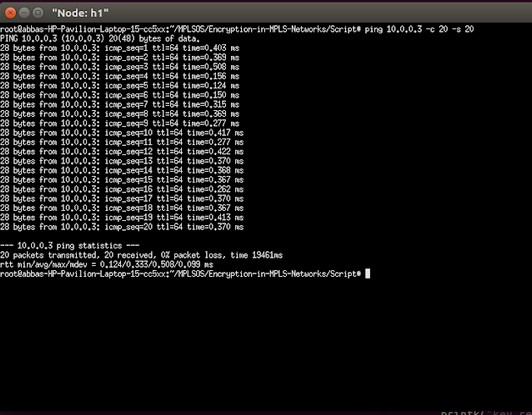
\includegraphics[width=\textwidth]{Final/MPLSOS_Small.jpg}
       \caption{MPLSOS RTT test with small packets}
       \label{fig:compbest}
\end{figure}

\begin{figure}
       \centering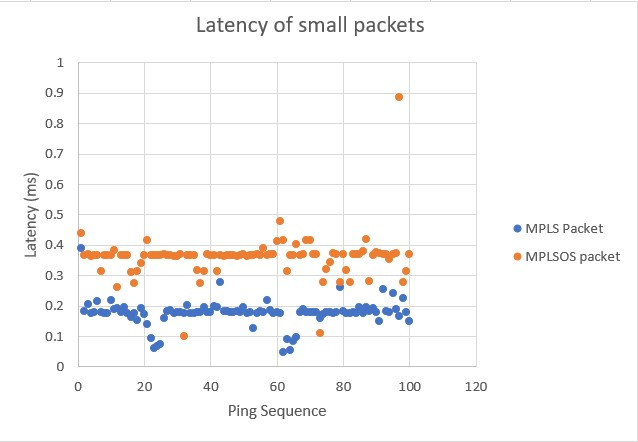
\includegraphics[width=\textwidth]{Final/Latency_small.jpg}
       \caption{RTT comparison of small packets}
       \label{fig:compbest}
\end{figure}


Figure 4.2 shows the RTT comparison of small packets with a minimum payload. The blue dots represents latency of normal MPLS packets and orange dots represents MPLS OS packets.
From Figure 4.1 and 4.2, We can see that the average RTT of normal MPLS packets are just below 0.2 ms and that of MPLS OS packets are just below 0.4 ms which is almost double to the first one.\\


\begin{figure}
       \centering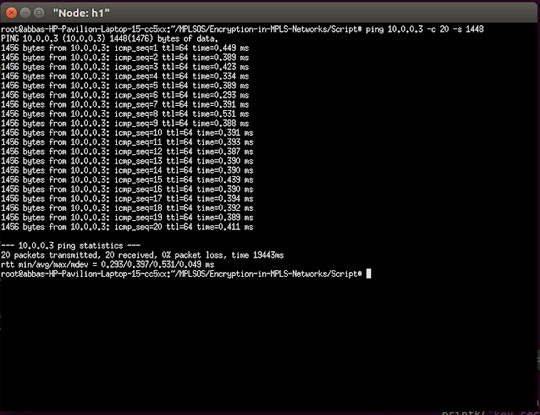
\includegraphics[width=\textwidth]{Final/MPLSOS_Large.jpg}
       \caption{MPLSOS RTT test with large packets}
       \label{fig:compbest}
\end{figure}

\begin{figure}
       \centering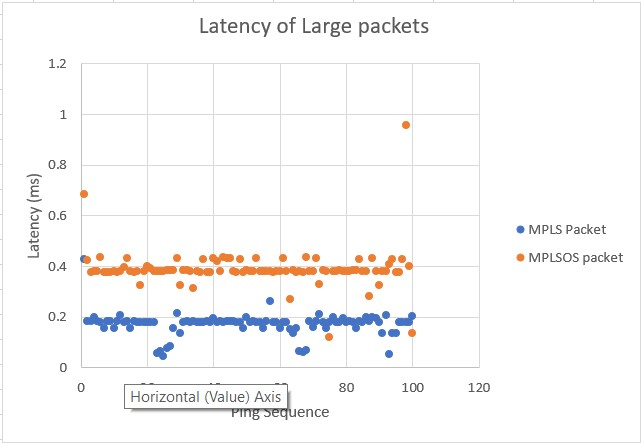
\includegraphics[width=\textwidth]{Final/Latency_large.jpg}
       \caption{RTT comparison of large packets}
       \label{fig:compbest}
\end{figure}


Figure 4.4 shows the latency comparison of Large packets with and without MPLS OS. The packets in the wire was exactly 1514 which is the MTU. Surprisingly the latency of large packets was very similar to small packets and I believe this is because of the emulation environment and behaviour will be different in the real hardware case.\\

\begin{figure}
       \centering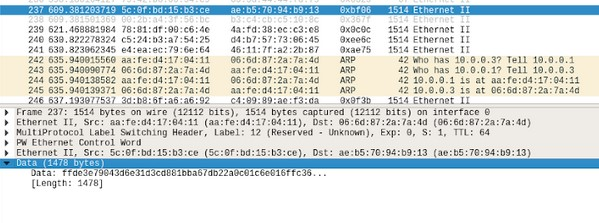
\includegraphics[width=\textwidth]{Final/mplsos_1514.jpg}
       \caption{1514 bytes MPLSOS Packet}
       \label{fig:compbest}
\end{figure}

Finally my finding is that there will be almost 50 percent performance reduction if we use MPLS OS between 2 adjacent LSRs(Hope by Hope) and the performance degradation will be less when we use MPLS OS as an end to end solution in a large MPLS Cloud. To get the exact figure of performance degradation, a real hardware deployment and testing of MPLS OS is required.\\

\subsection{MTU Limitation}

We know that unlike IP Packets, MPLS packet doesn’t undergo IP Fragmentation if the packet size exceeds the MTU. MTU is the maximum size of the frame the layer 2 can accept and the packet is consisting of payload and headers. If we use MPLS, it will add 4 bytes to the frame per labels pushed. If we push 2 labels, it will add 8 bytes. In MPLS OS, we add a CW Header which 4 bytes in size and a 4 bytes header MEL apart from the label. The cipher text (encrypted payload) of MPLS OS larger than plain text payload. So the packet going out of an MPLS OS Router will be much larger than the incoming packet and much care should be given here to make sure that overall packet size shouldn’t exceed the MTU. I kept the MTU of the experiment setup as 1514 byes and I tested a packet with 1515 bytes and the result was the packet got dropped by the LSR which was expected. \\


\begin{figure}
       \centering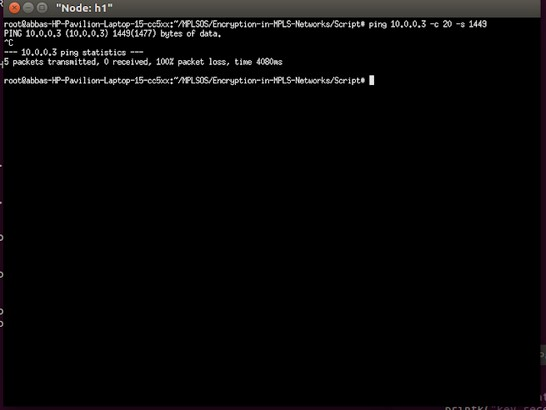
\includegraphics[width=\textwidth]{Final/MPLS_Frag.jpg}
       \caption{1515 bytes MPLSOS Packet}
       \label{fig:compbest}
\end{figure}